\section{\methodname: Natural Language as the Action Interface}
\label{sec:method}

Realizing the language-as-action-interface end-to-end requires
addressing two architectural challenges inherent to any language-conditioned,
multi-entity interactive world model:
($1$) \emph{Per-frame language conditioning} and ($2$)
\emph{Real-time long-horizon streaming inference}.
We contribute one principled solution for each, structuring our pipeline into two stages.
\textbf{Stage~$\mathbf{1}$} (Section~\ref{sec:stage1}) addresses per-frame language conditioning
via a per-entity prompt formulation on a bidirectional backbone with decoupled
text cross-attention.
\textbf{Stage~$\mathbf{2}$} (Section~\ref{sec:stage2}) achieves real-time long-horizon
streaming generation through a two-stage distillation (ODE initialization followed by
Self-Forcing) combined with RoPE-decoupled KV-cache sliding.
Throughout this work, the action interface targets the
\emph{discrete-semantic action} regime, 
where each per-frame action
admits a textual description; 
% while
continuous control signals (e.g., camera
$\mathrm{SE}(3)$ trajectories) are out of scope and discussed in
Appendix~\ref{app:limitations}.

%% ═══════════════════════════════════════════════════════════════
\subsection{Stage 1: Language-Conditioned Architecture}
\label{sec:stage1}

We adopt natural language as the action interface, which inherently 
decouples the conditioning signal from any specific engine or entity and 
thereby enables \textbf{generalization} across both entity types and world domains. 
Realizing this interface on top of a pretrained bidirectional video 
backbone~\citep{wang2025wan} requires three coupled design choices: 
($1$) how multi-entity prompts are formulated, 
($2$) how attention is structured to turn 
high-level prompts into frame-accurate actions, and ($3$) how positional 
indices are assigned so that both training and bounded streaming inference 
stay in distribution.
% As discussed in Section~\ref{sec:intro}, device-level inputs are poorly suited to independently conditioning several heterogeneous entities, and discrete action IDs offer little semantic structure for cross-entity generalization. We therefore adopt natural language as the action interface. This subsection covers three coupled design choices: how prompts are formulated, how attention is structured to turn high-level prompts into frame-accurate actions, and how positional encodings are assigned so that both training and bounded inference stay in distribution.

\paragraph{Prompt Formulation. }
We represent multi-entity actions as a structured natural-language prompt with parallel, 
syntactically isolated slots (one per entity) at a $0.25$\,s granularity. As a concrete example, for two-entity control:
% Each 0.25\,s action window is described by a structured natural-language prompt with two parallel, syntactically isolated slots:
\begin{center}
  \small\texttt{Player performs [ACTION\_P]. Boss performs [ACTION\_B].}
\end{center}
This template supports both \textbf{simultaneous control} and 
\textbf{entity decoupling}: the temporal alignment of the two slots encourages the 
model to reason jointly about inter-entity dynamics within each frame, while the 
syntactic separation preserves independent control pathways for each entity. 
The template also extends naturally to settings with more or fewer entities 
by simply appending or omitting slots, requiring \textbf{no architectural modification}
and demonstrating the inherent \textbf{scalability} of the natural-language interface.

% \paragraph{Passive-Response Exclusion.}
% Passive physiological responses, in our setting taking-hit events, are not 
% deliberate actions issued by the controller, but involuntary responses 
% to external events happening to an entity. 
% Including them in the conditioning space introduces involuntary pauses that 
% corrupt the model's understanding of volitional movement. 
% We therefore exclude all such passive-response labels from the prompt vocabulary: the prompt vocabulary describes \emph{what an entity chooses to do}, not what happens to it.
% \paragraph{Excluding passive-response events from the prompt vocabulary.}
% Passive physiological responses---in our setting, taking-hit events---are not deliberate actions the controller issues but involuntary responses to events happening to an entity. Including them in the conditioning space introduces involuntary pauses that corrupt the model's understanding of volitional movement. We therefore exclude all such passive-response labels from the prompt vocabulary: the prompt vocabulary describes \emph{what an entity chooses to do}, not what happens to it.

\begin{figure*}[t]
    \centering
    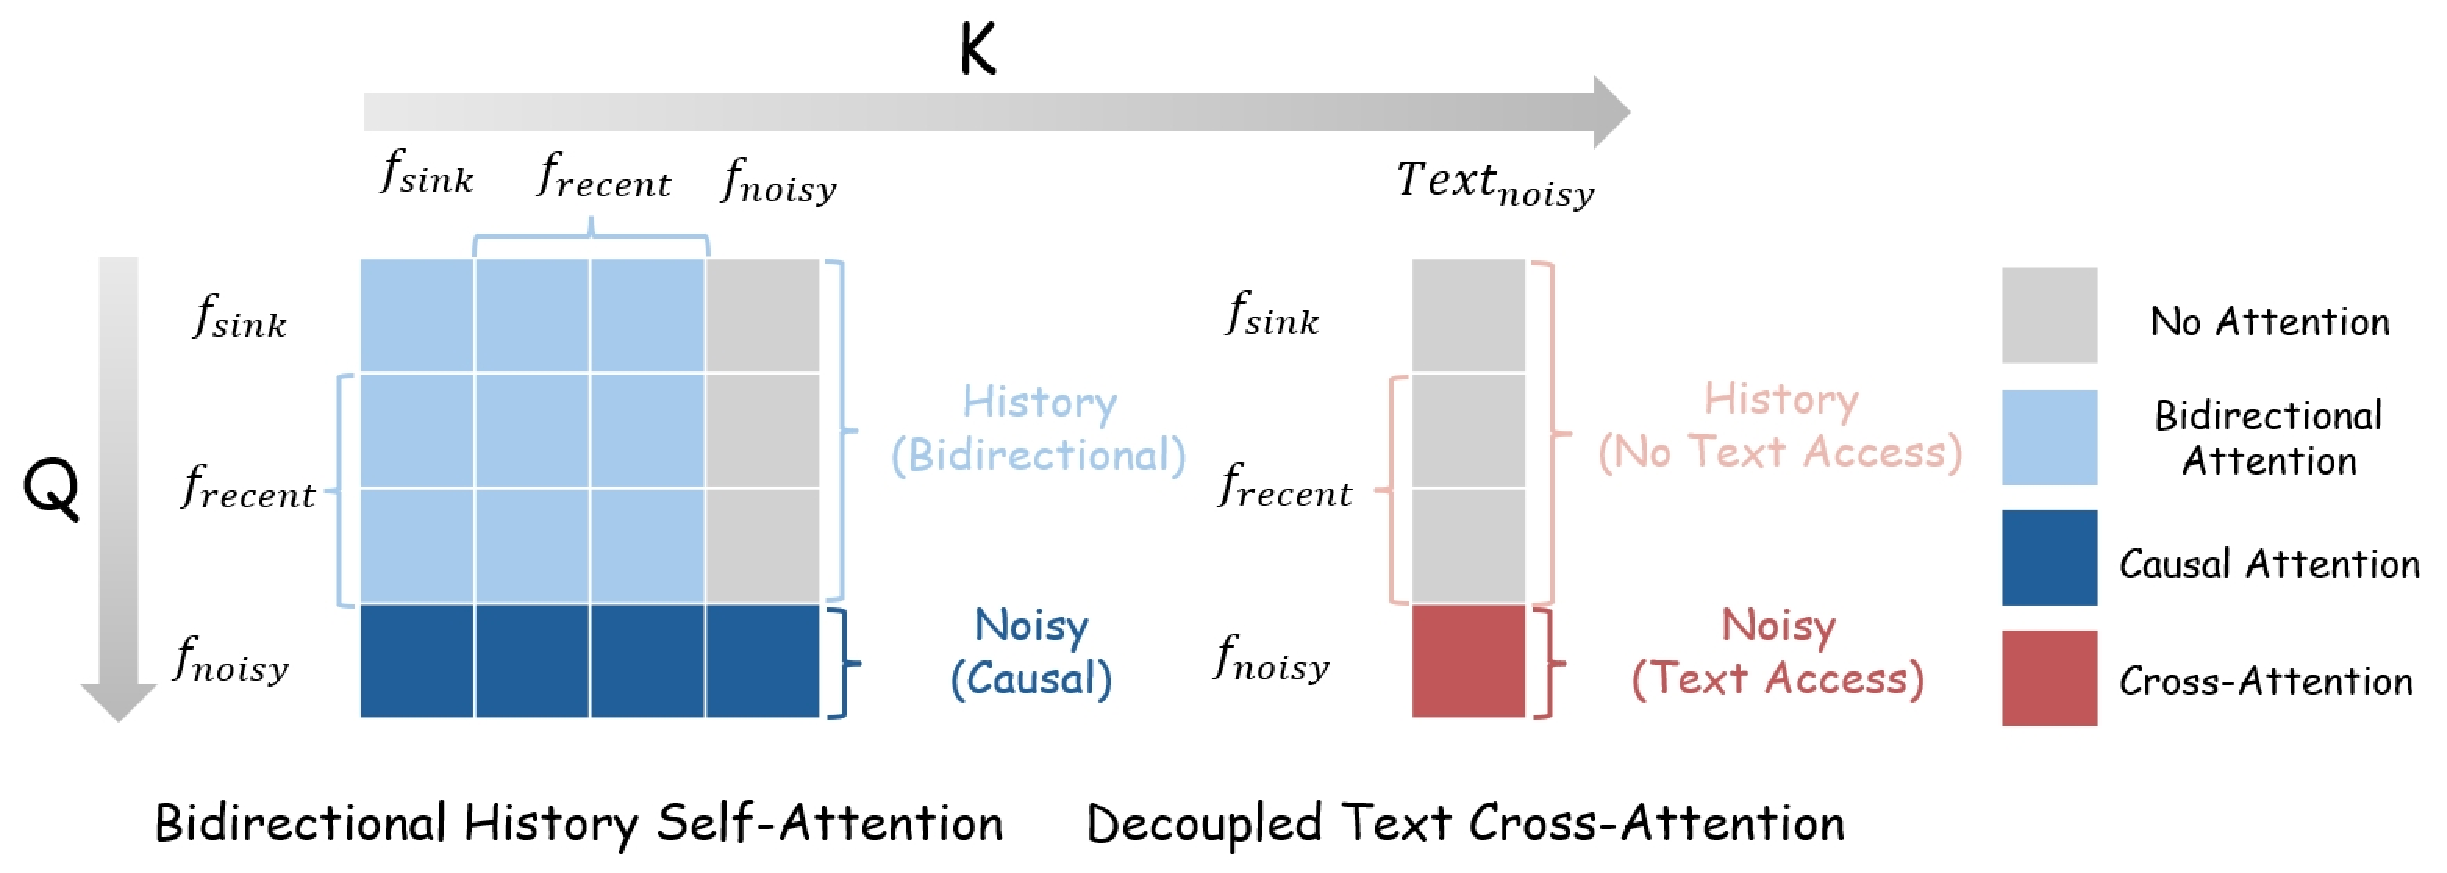
\includegraphics[width=\linewidth]{figures/fig_masked_attention.pdf}
    \caption{\textbf{Attention design.} Bidirectional self-attention is retained over history frames to preserve the spatio-temporal priors of the pretrained base model. Action cross-attention is restricted exclusively to the noisy target frame, preventing temporal cross-contamination. Together, these two constraints improve per-frame controllability without degrading generation quality.}
    \label{fig:masked_attention}
\end{figure*}

\paragraph{Context Assembly. }
In the autoregressive diffusion-based video generation framework,
each target frame is denoised by attending
to a context window of conditioning frames passed as clean latents.
We organize this window using a \emph{Sink + Recent + Noisy} context structure;
for each training step targeting frame~$t$:
% We adopt a \emph{Sink + Recent + Noisy} context structure. For each training step targeting frame~$t$:
\begin{itemize}[leftmargin=*,topsep=2pt,itemsep=1pt]
  \item \textbf{Sink frame} ($K_s{=}1$): the first frame of the episode, anchoring global context (arena geometry, character appearance) following the attention-sink mechanism of~\citet{xiao2023streamingllm}.
  \item \textbf{Recent frames} ($K_r{=}7$): the $7$ most recent clean latent tokens preceding $t$. Each latent token corresponds to $0.25$\,s of gameplay after the base model's VAE temporal compression, so the recent context spans $1.75$\,s of game time. We ablate $K_r$ in Appendix~\ref{app:stage2_ablation}.
  \item \textbf{Noisy target} ($K_n{=}1$): the partially-denoised latent of frame $t$.
\end{itemize}

\paragraph{Per-Frame Language-Conditioned Attention. }
The conventional approach, with causal self-attention over all visual tokens plus full text cross-attention, introduces two failure modes under per-frame language conditioning:
\textbf{($\mathbf{1}$)~Destruction of pretrained priors.} The Wan~$2.2$ base model was pretrained with full bidirectional attention; its weights encode symmetric co-occurrence statistics. Imposing a global causal mask discards these priors, requiring costly re-adaptation.
\textbf{($\mathbf{2}$)~Temporal cross-contamination.} Each action prompt $a_t$ describes exclusively what occurs at time~$t$. Allowing $a_t$ to cross-attend to history frames causes it to retroactively corrupt committed past representations, producing spurious action echoes in adjacent frames.
We address both issues with a dedicated attention mechanism for
per-frame language conditioning (Figure~\ref{fig:masked_attention}):
\textbf{($\mathbf{1}$) Bidirectional history attention.}
We apply \textit{full bidirectional self-attention} over the $(K_s + K_r)$ history tokens, preserving the base model's pretrained co-occurrence statistics. A causal boundary separates history from the noisy target, enforcing correct temporal ordering at generation time.
\textbf{($\mathbf{2}$) Decoupled text cross-attention.}
The per-frame action prompt $a_t$ cross-attends \emph{exclusively} with the noisy target token; history frames are masked out entirely. This prevents temporal cross-contamination: the current annotation cannot influence committed past representations. Ablation study appears in Appendix~\ref{app:stage1_ablation}.

\paragraph{Bounded RoPE Position Assignment.}
\label{sec:rope_design}
The naive sequential position assignment lets token indices grow
unboundedly during streaming inference, placing them outside the range
seen during training; this is a \textbf{RoPE out-of-distribution (OOD)} problem
that fundamentally breaks long-horizon generation.
We instead introduce two independent bounds: a sliding window size
$K_r$ (how many recent frames the KV cache holds) and a position cap
$C\ge K_r$ (the largest local RoPE index any token can receive).
The sink frame is permanently anchored at position $0$, the noisy
target at $\min(p_t, C)$ where $p_t$ is its absolute frame index, and
the $K_r$ recent frames occupy the consecutive positions immediately
preceding the target.
$K_r$ caps per-step compute and memory; $C$ caps the positional range
exposed to the model, and is set so every position used at inference
also occurs during training. Together the two prevent RoPE OOD and
enable the KV-cache sliding mechanism at inference (Section~\ref{sec:stage2}).
% The sink frame is assigned fixed position~0; recent frames receive sliding positions $1,\ldots,K_r$; the noisy target receives $K_r{+}1$. This scheme is \emph{bounded}: every token always carries a position in $\{0,\ldots,8\}$, the range seen during training. This guarantee serves double duty: it prevents RoPE OOD during training \emph{and} enables the KV-cache sliding mechanism at inference (Section~\ref{sec:stage2}).

\paragraph{Training Setup. }
We fine-tune Wan~$2.2$ TI2V-5B~\citep{wang2025wan} end-to-end on $16$ H100 GPUs
using Fully Sharded Data Parallel (FSDP) and mixed-precision training.
We employ a two-resolution curriculum: $1{,}000$ warmup steps at $256{\times}448$
(learning rate $2\!\times\!10^{-5}$), followed by $50{,}000$ steps at
$480{\times}832$ (learning rate $1\!\times\!10^{-5}$), with a global batch
size of $64$.
Training data are described in Section~\ref{sec:setup}.
% We fine-tune Wan~2.2 TI2V-5B~\citep{wan2025} end-to-end on 64$\times$H100 GPUs with FSDP and mixed precision. Training uses a two-resolution curriculum: 256$\times$448 for 1{,}000 warm-up steps (lr\,$=2\!\times\!10^{-5}$), then 480$\times$832 for 29{,}000 steps (lr\,$=1\!\times\!10^{-5}$), with global batch size 64. The training data is described in Section~\ref{sec:data_pipeline}.

%% ═══════════════════════════════════════════════════════════════
\subsection{Stage 2: Real-Time Streaming Inference}
\label{sec:stage2}

Real-time streaming inference is a prerequisite for any world model that aspires to support genuine interaction. The Stage~$1$ bidirectional teacher, however, requires $50$ denoising steps per frame and attends over a full visual context, neither of which is compatible with real-time play. Stage~$2$ addresses two coupled bottlenecks for this challenge: ($1$) reducing per-frame compute via distillation, and ($2$) bounding per-frame memory via KV-cache sliding while preserving positional coherence.
% The bidirectional teacher from Stage~1 requires ${\sim}$20 denoising steps per frame and attends over a full visual context, making real-time play infeasible. Stage~2 addresses two coupled bottlenecks: reducing per-frame compute via distillation, and bounding per-frame memory via KV-cache sliding while preserving positional coherence.

% \subsubsection*{ODE-Initialized Self-Forcing Distillation}
% We distill the teacher into a 2-step causal student in 
% two sub-stages: (1) ODE initialization to reconcile the bidirectional-to-causal
% attention mismatch, and (2) Self-Forcing for step reduction.
% We distill the teacher into a 2-step causal student in two sub-stages.

\paragraph{ODE Initialization Before Distillation.}
The teacher was pretrained with bidirectional history attention,
which grants rich spatio-temporal priors but is fundamentally incompatible with
the strictly causal attention required by streaming inference.
Before distillation, we must reconcile this mismatch. 
We initialize a causal student from the teacher's weights and align their 
predicted velocity fields via a flow-matching consistency
objective~\citep{lipman2022flow}:
\begin{equation}
  \mathcal{L}_{\text{ODE}} = \mathbb{E}_{\tau,v_0,\epsilon}\bigl[\|f_\theta(v_\tau;\,\text{causal}) - f_{\text{teacher}}(v_\tau;\,\text{bidir})\|_2^2\bigr].
\end{equation}
In practice,
this objective closes the attention-mask gap within $1{,}000$ steps at 
$480{\times}832$ resolution ($16$ H100 GPUs, learning rate\,$=5\!\times\!10^{-6}$, batch size $128$).
% \paragraph{ODE Initialization.}
% We initialize a causal student from the teacher's weights and align its predicted velocity field via a flow-matching consistency objective~\citep{lipman2022flow}:
% \begin{equation}
%   \mathcal{L}_{\text{ODE}} = \mathbb{E}_{\tau,v_0,\epsilon}\bigl[\|f_\theta(v_\tau;\,\text{causal}) - f_{\text{teacher}}(v_\tau;\,\text{bidir})\|_2^2\bigr]
% \end{equation}
% This resolves the attention-mask mismatch in 1{,}000 steps at 480$\times$832 (64$\times$H100, lr\,$=5\!\times\!10^{-6}$, batch size 128).

\paragraph{Self-Forcing Distillation.}
Building on the ODE-initialized student, 
we apply Self-Forcing~\citep{chen2025selfforcing} distillation to reduce inference to just
\textbf{$\mathbf{2}$ steps}. During training, the student conditions on \emph{its own
previously generated frames} rather than ground-truth frames, 
directly suppressing the compounding errors that 
would otherwise accumulate over autoregressive rollout.
% Starting from the ODE-initialized student, Self-Forcing~\citep{chen2025selfforcing} collapses inference to \textbf{2 steps}. During training the student conditions on its \emph{own} previously generated frames, directly suppressing the compounding errors that would otherwise accumulate during extended play.

\paragraph{RoPE-Decoupled KV-Cache Sliding Window. }
\label{sec:rope_decouple}
Under the bounded RoPE scheme in \Cref{sec:stage1} for OOD prevention, 
a bounded KV-cache sliding window is required to enable real-time streaming inference. 
However, the bounded relative positional indices are
time-dependent: 
after each eviction, surviving keys must be reassigned updated local 
relative positions. 
If RoPE-rotated keys are cached, their embeddings remain anchored to stale
indices and become inconsistent with the current query, causing temporal
flickering in the generated video. 
We therefore cache raw keys \emph{before} RoPE rotation and apply RoPE on-the-fly
with up-to-date local relative positions. 
Let $p^{\text{abs}}_i$ and $p^{\text{abs}}_t$ denote the absolute positions of 
cached frame $i$ and the current query $t$, respectively, with $C$ the local position cap defined in \Cref{sec:rope_design}.
Our local relative position assignment and RoPE-decoupled attention are:
\begin{align}
  p^{\text{local}}_i &= \text{clamp}\!\bigl(p^{\text{abs}}_i - \delta,\; 0,\; C\bigr),
    \quad \delta = \max\!\bigl(0,\, p^{\text{abs}}_t - C\bigr). \label{eq:local_pos} \\
  \text{Attn}(q_t, k_i) &= \text{Softmax}\{\bigl(q_t \cdot R(p^{\text{local}}_t)\bigr)
    \bigl(k_i^{\text{raw}} \cdot R(p^{\text{local}}_i)\bigr)^\top / \sqrt{d} \}.
  \label{eq:rope_decouple}
\end{align}
When the buffer is full, the oldest non-sink frame is evicted while the sink frame is
permanently retained at $p_{\text{sink}}^{\text{local}}{=}0$. The clamp cap $C$
keeps every local position within the range exercised during training,
ensuring long-horizon generation remains fully OOD-free. 
Together, our design guarantees: (a)~$\mathcal{O}(K_s + K_r)$ bounded memory;
(b)~all positions in-distribution; (c)~artifact-free evictions.
% Unbounded generation requires bounding VRAM while preserving positional coherence. Naive truncation causes flickering when evicted frames' absolute position indices suddenly disappear. We solve this by storing keys \emph{before} RoPE rotation and applying rotation on-the-fly using local positions:
% \begin{align}
%   p^{\text{local}}_i &= \text{clamp}\!\bigl(p^{\text{abs}}_i - \delta,\; 0,\; C\bigr), \quad \delta = \max\!\bigl(0,\, p^{\text{abs}}_{\text{current}} - C\bigr) \label{eq:local_pos} \\
%   \text{Attn}(q_t, k_i) &= \bigl(q_t \cdot R(p^{\text{local}}_t)\bigr)\bigl(k_i^{\text{raw}} \cdot R(p^{\text{local}}_i)\bigr)^\top / \sqrt{d}
%   \label{eq:rope_decouple}
% \end{align}
% When the buffer is full, the oldest non-sink frame is evicted; the sink entry is permanently retained. Because the sliding window bounds relative positions to $[0, K_r{+}1]{=}[0, 8]$---exactly the training range established by the RoPE design in Stage~1---long-horizon generation never encounters OOD positions. The local cap $C{=}16$ is a clamping bound; in practice, actual relative positions remain within $[0, 8]$. Together: (a)~VRAM is bounded to $\mathcal{O}(K_s + K_r)$; (b)~all positions stay in-distribution; (c)~evictions produce no visible artifacts.

